\documentclass[letterpaper,10pt,serif,draftclsnofoot,onecolumn,compsoc,titlepage]{IEEEtran}

\usepackage{graphicx}                                        
\usepackage{amssymb}                                         
\usepackage{amsmath}                                         
\usepackage{amsthm}                                          
\usepackage{cite}
\usepackage{alltt}                                           
\usepackage{float}
\usepackage{color}
\usepackage[hyphens]{url}
\usepackage{pgfgantt}
\usepackage{rotating}
\usepackage{enumitem}
\usepackage{array}
\usepackage{gensymb}
\usepackage[T1]{fontenc}
\usepackage{balance}
\usepackage[TABBOTCAP, tight]{subfigure}
\usepackage{enumitem}
\usepackage{subfiles}
\usepackage{pdfpages}

\usepackage{geometry}
\geometry{margin=.75in}
\usepackage{hyperref}
\usepackage{breakurl}
%\usetikzlibrary{shapes, positioning, calc}
\usepackage{caption}
\usepackage{listings}
%\usepackage[utf8]{inputenc}
%pull in the necessary preamble matter for pygments output

\newcommand{\subparagraph}{}
\usepackage{titlesec}
\usepackage{titletoc}
\setcounter{secnumdepth}{5}
\setcounter{tocdepth}{5}
\titleformat{\paragraph} [hang] {\normalfont\normalsize\bfseries} {\theparagraph} {1em} {}

\usepackage{listings}
\definecolor{dkgreen}{rgb}{0,0.6,0}
\definecolor{gray}{rgb}{0.5,0.5,0.5}
\definecolor{mauve}{rgb}{0.58,0,0.82}

\lstset{
  %frame=tb,
  language=C++, %added
  aboveskip=3mm,
  belowskip=3mm,
  showstringspaces=false,
  columns=flexible,
  basicstyle={\small\ttfamily},
  numbers=none,
  %added
  backgroundcolor=\color{black!5}, % set backgroundcolor
  basicstyle=\footnotesize,% basic font setting
  %added
  breaklines=true,
  breakatwhitespace=true,
  tabsize=4
}

%% The following metadata will show up in the PDF properties
\hypersetup{
   colorlinks = true,
   citecolor = black,
   linkcolor = black,
   urlcolor = black,
   breaklinks = true,
   pdfauthor = {Shu-Ping Chien, Brock Smedley, W Keith Striby Jr},
   pdfkeywords = {CS463 "Senior Project" Final Report},
   pdftitle = {CS463 Final Report},
   pdfsubject = {CS463 Final Report},
   pdfpagemode = UseNone
}

\parindent = 0.0 in
\parskip = 0.1 in
\title{Final Report: Multi-Camera, SoM Based, Real-Time Video Processing for UAS and VR/AR Applications}
\author{Area 51: Shu-Ping Chien, Brock Smedley, W Keith Striby Jr \\ 12 June 2018 \\ CS463, Senior Software Engineering Project, Spring 2018}


\begin{document}
\begin{titlepage}
\maketitle

\begin{abstract}

Write me \\


\thispagestyle{empty}
\end{abstract}
\end{titlepage}

\newpage
\tableofcontents

\newpage

\section{Project Introduction}

\subsection{Problem}
% talk about 1) what's being requested, 2) who requested it & why, & its importance
% 2-3 paragraphs, minimum

\subsection{Persons Involved and Their Role}
% talk about: 1) members of the team, roles, restate client & state his role

\newpage 

\section{Requirements Document}

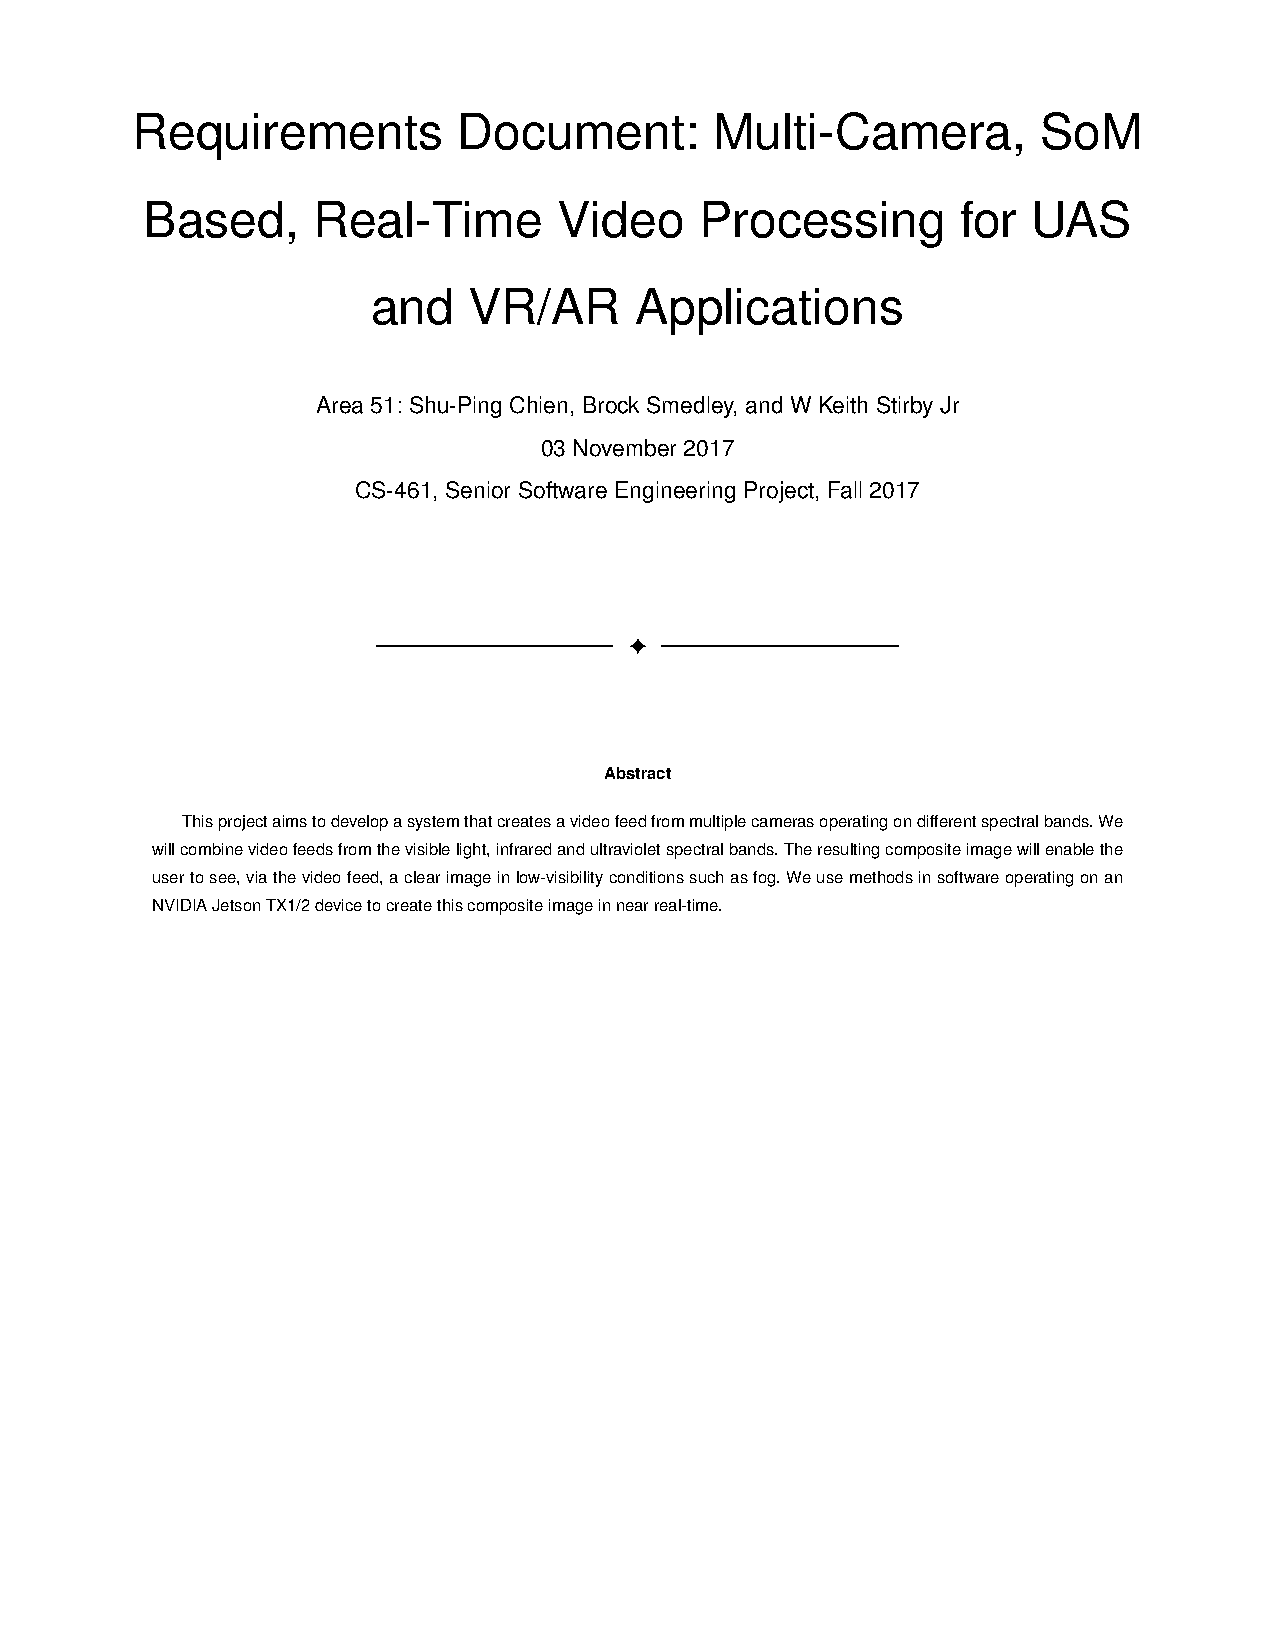
\includepdf[pages={1,2,3,4,5,6,7,8}]{documents/requirements_group51.pdf}

\section{Design Document}

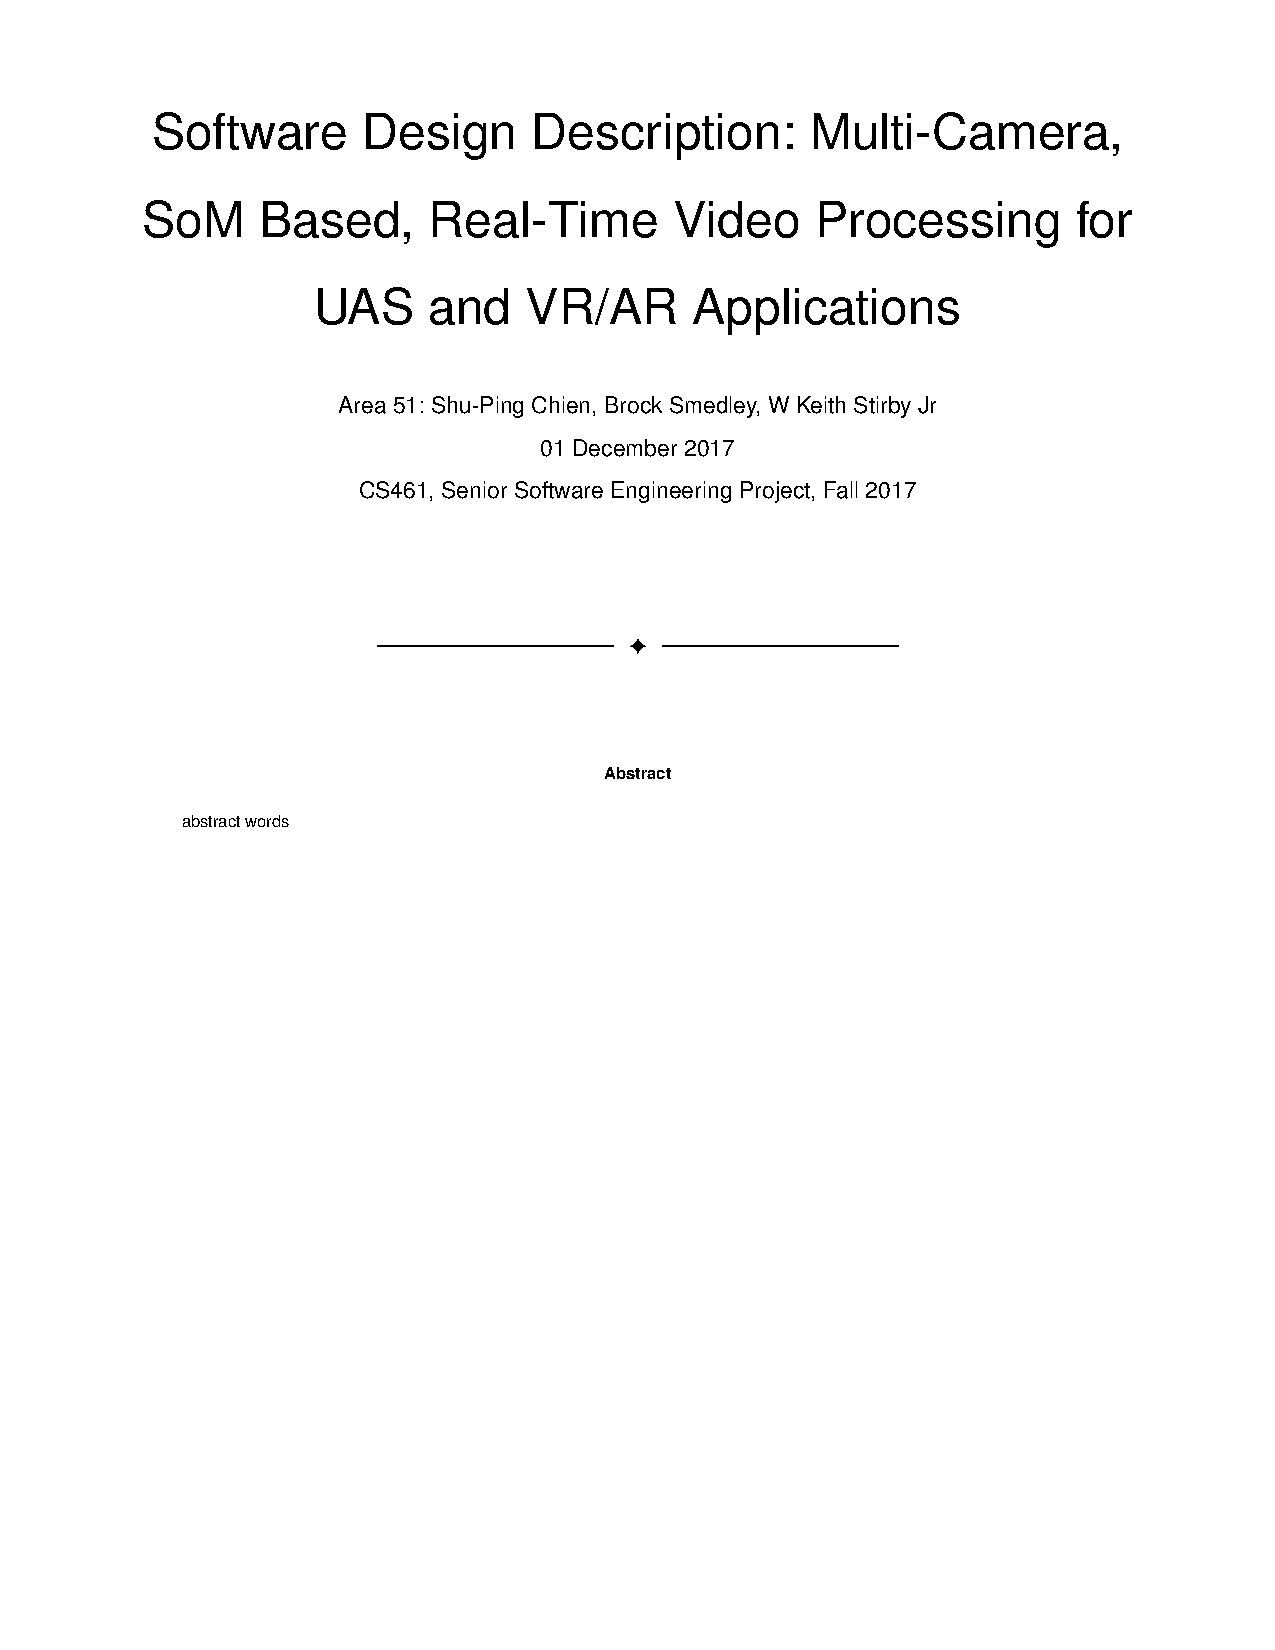
\includepdf[pages={1,2,3,4,5,6,7,8}]{documents/SDD_Group51.pdf}

\newpage

\section{Technology Reviews}

\subsection{Shu-Ping's Technology Review}

%\input{documents/Technology_Review/}

\newpage

\subsection{Brock Smedley's Technology Review}

%\input{documents/smedleyTR}

\newpage

\subsection{Keith Striby's Technology Review}

\includepdf[pages={1,2,3,4,5,6,7,8,9,10,11,12,13}]{documents/Technology_Review_Striby.pdf}

\section{Weekly Blog Posts}


\newpage

\section{Final Poster}


\newpage

\section{Project Documentation}


\newpage

\section{Recommended Technical Resources for Learning More}


\newpage

\section{Conclusions and Reflections}


\newpage

\section{Appendix 1: Essential Code Listings}
% doesn't have to be everything, but there should be stuff here for someone to learn from


\nocite{*}
\newpage
\bibliographystyle{ieeetr}
\bibliography{PFPR_Group51}
\end{document}
